%%%%%%%%%%%%%%%%%%%%%%%%%%%%%%%%%%%%%%%%%%%%%%%%%%%%%%%%%%%%%%%%%
\section{Introduction}\label{sec:1}

\subsection[Research background]{Research background}\label{subsec:1-1}
\begin{frame}
\frametitle{\normalsize{Background}}\transwipe
      % \breference
      % [1] E. Fridman, ``Introduction to Time-Delay Systems: Analysis and Control,''  \emph{Springer,} pp.~22-28, 2014.
      % \ereference
 \begin{itemize}
  \item With the rapid development of wireless communication technology, various kinds of large-scale network systems are increasingly applied in the fields of engineering technology. Thus, comes the problem of how to make interconnected multi-agent work together.
  \vspace{0.4cm}
  \begin{columns}[c]
 \column{6cm}
   \begin{figure}
       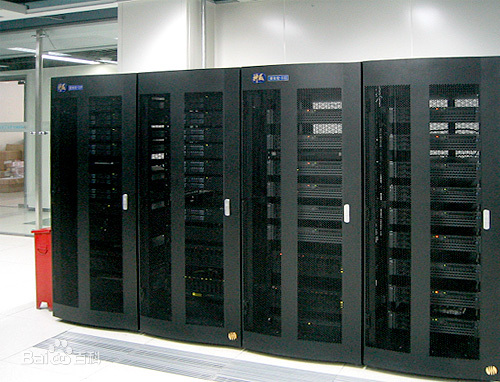
\includegraphics[height=0.7in]{figure/game/1-computer_cluster.jpg}
       \vspace{-6pt}
       \caption{computer clusters}
      \label{fig1}
   \end{figure}
    \column{6cm}
    \begin{figure}
      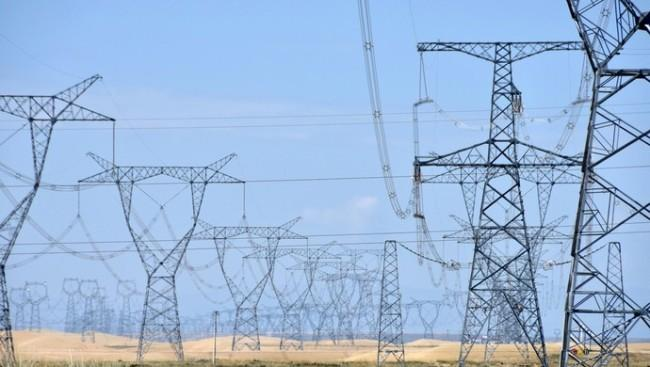
\includegraphics[height=0.7in]{figure/game/2-multi-microgrid.jpeg}
      \vspace{-6pt}
      \caption{multi-microgrid systems}
     \label{fig2} 
  \end{figure}
    \end{columns}

  \begin{columns}[c]
    \column{6cm}
      \begin{figure}
          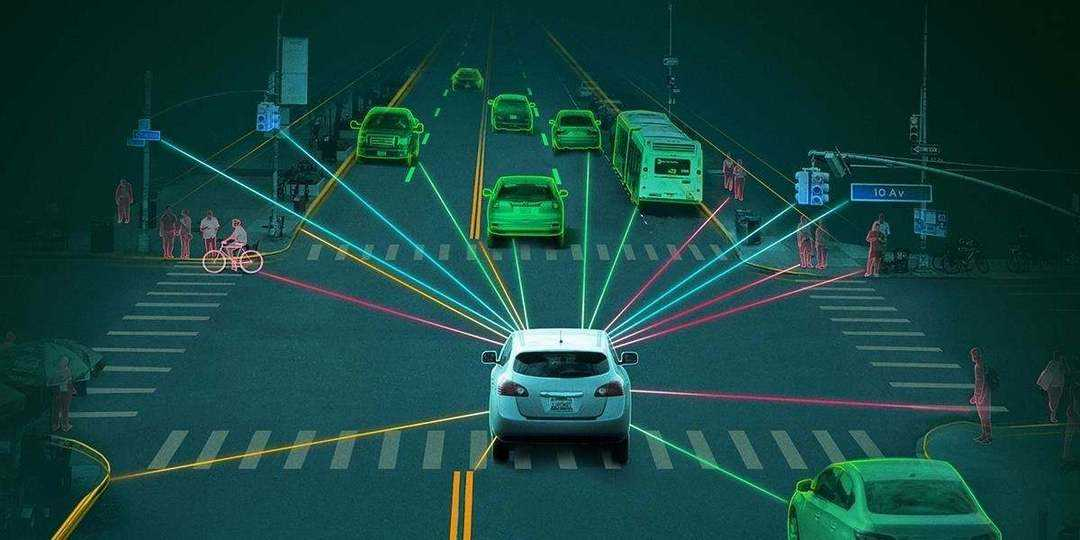
\includegraphics[height=0.7in]{figure/game/3-autonomus-driving.jpeg}
          \vspace{-6pt}
          \caption{autonomous driving networks}
         \label{fig3}
      \end{figure}
       \column{6cm}
       \begin{figure}
         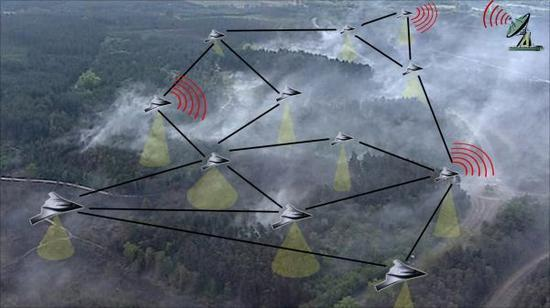
\includegraphics[height=0.7in]{figure/game/4-UAV-systems.jpeg}
         \vspace{-6pt}
         \caption{UAV systems}
        \label{fig4} 
     \end{figure}
       \end{columns}

  \end{itemize}
\end{frame}

\subsection[Game Theory]{Game theory in multi-agent}\label{subsec:1-2}

\begin{frame}
\frametitle{\normalsize{Game theory in multi-agent}}\transwipe

\begin{itemize}
\item \textcolor[rgb]{0.00,0.00,1.00}{Game theory}, which studies the cooperation and conflict among multiple rational decision makers, called players, can be utilized to analyze a large class of engineering system.
\item In general multi-agent problems, the global cost function as follows. $f_i(x)$ is the local cost function depends on $x_i$, we try to minimize global cost function.
\vspace{6pt}
\begin{equation}
\begin{split}
 J(x)=\sum_{i=1}^N f_i(x), x=\left[x^1, \ldots, x^m\right]^T \in \mathbb{R}^m
\end{split}
\end{equation}

\item In game theroy problems, the players’ objective functions are dependent on \textcolor[rgb]{0.00,0.00,1.00}{other players’ actions}, which lead to the coupling between the players’ actions in the decision-making process. 
 \vspace{6pt}
 \begin{equation}
 \begin{split}
  \min _{x_i \in \mathbb{R}_i} J_i\left(x_i, x_{-i}\right), \quad \text { s.t. } \quad x_i \in X_i \end{split}
 \end{equation}
\end{itemize}
\breference
\scriptsize
[1]Z. M. Fadlullah, "A survey of game theoretic approaches in smart grid," WCSP, 2011, pp. 1-4.\par
\ereference
\end{frame}


\begin{frame}
\frametitle{\normalsize{Nash Equilibrium}}\transwipe
\begin{itemize}

\item An action $x^\star$ is defined as an \textcolor[rgb]{0.00,0.00,1.00}{Nash Equilibrium} of the game G(N, $J_i$), if for all i $\in N$
\begin{equation}
  J_i\left(x_i^*, x_{-i}^*\right) \leq J_i\left(x_i, x_{-i}^*\right)
\end{equation}
Let $x_i$ be player i's action and $x_{-i}$ represent other players’ actions.
\vspace{6pt}

\item From the above definition, none of the agents can benefit from \textcolor[rgb]{0.00,0.00,1.00}{unilaterally} changing its strategy at NE conditions.
\vspace{6pt}

\item Because if one player changes it's strategy, others will also change their strategies, which leads to a increasement of cost function. 

% \item In order to reach NE, every agent needs to consider the actions of other agents.


\end{itemize}

% Let $\beta \geq r \geq 0$ be given real numbers($\beta$ may be $+\infty$), $E^n$ be an n-dimensional linear vector space with a seminorm $|\cdot|$, $p:[-\beta,0]\to (0, \infty)$ be Lebesque integrable on $[-\beta,0]$, positive and nondecreasing on $[-\beta,0]$.Let $\mathcal{B}=\mathcal{B}([-\beta,0], E^n)$ be the Banach sapce of functions which are continuous on $[-r,0]$ and such that 
% \begin{equation}
% |\phi|=\sup_{\theta \in [-r,0]}|\phi(\theta)|+\int^0_{-\beta}p(\theta)|\phi(\theta)|d\theta <\infty
% \end{equation}
\end{frame}
